\subsection{Documenti per l'esperimento}
In questa sezione vengono presentati e descritti in dettaglio tutti i documenti, i moduli e i questionari utilizzati durante lo svolgimento dell'esperimento. Di seguito verranno illustrati gli strumenti sottoposti a ciascun utente e il materiale a supporto dello sperimentatore, spiegandone la specifica funzione all'interno delle diverse fasi del test.

\subsubsection{Checklist per lo sperimentatore}
Per assicurarsi che ogni sessione di test si svolgesse in modo uniforme, è stata redatta una \textit{checklist} a uso esclusivo dello sperimentatore. Questo documento ha permesso di standardizzare le procedure, fornendo una guida strutturata per la gestione ottimale dei test. Le attività delineate nella checklist sono state suddivise in quattro fasi dell'esperimento distinte:

\begin{itemize}
    \item Prima di accogliere l'utente (\textbf{Preparazione})
    \item Prima dell'esperimento (\textbf{Introduzione})
    \item Durante l'esperimento (\textbf{Esecuzione})
    \item Dopo l'esperimento (\textbf{Debriefing})
\end{itemize}

\begin{table}[H]
  \centering
  \small
  \renewcommand{\arraystretch}{1.5}
  \begin{tabularx}{\textwidth}{|>{\raggedright\bfseries\arraybackslash}p{3.5cm}|>{\raggedright\arraybackslash}X|}
    \hline
    \rowcolor{gray!30}
    \multicolumn{2}{|c|}{\textbf{CHECKLIST}} \\
    \hline
    Prima di accogliere l'utente &
    \vspace{-8pt}
    \begin{itemize}[itemsep=2pt, topsep=2pt, parsep=0pt]
        \item navigare sul drive e scaricare il materiale necessario
        \item caricare i file necessari su BrainBox
        \item attivare il tool per il conteggio del numero di click
        \item nel caso in cui si usassero i seed, eseguire il comando \verb|php artisan migrate:fresh --seed| (solo la prima volta)
        \item Per versione A: eseguire i comandi \verb|npm run dev| e \verb|php artisan serve|
        \item Per versione B: eseguire il comando \verb|dev.bat| su windows e \verb|./dev.sh| su linux
    \end{itemize}
    \vspace{-6pt} \\
    \hline
    Prima dell'esperimento &
    \vspace{-8pt}
    \begin{itemize}[itemsep=2pt, topsep=2pt, parsep=0pt]
        \item salutare l'utente e ringraziarlo per la disponibilità
        \item sottolineare che l'esperimento è volto alla valutazione del sito
        \item garantire la riservatezza dei dati richiesti e dei risultati
        \item descrivere la struttura generale dell'esperimento
        \item indicare la possibilità di abbandonare il task se reputato troppo difficile
        \item far compilare il questionario dell'anagrafica, ribadendo la riservatezza dei dati
        \item consegnare all'utente il questionario di valutazione da comiplare durante il test
        \item aprire il modulo per lo sperimentatore da compilare in parallelo al questionario di valutazione dell'utente
    \end{itemize}
    \vspace{-6pt} \\
    \hline
    Durante l'esperimento &
    \vspace{-8pt}
    \begin{itemize}[itemsep=2pt, topsep=2pt, parsep=0pt]
        \item tenere conto del numero di errori, del numero di click e del tempo in cui viene eseguito un singolo compito o scenario
        \item se l'utente chiede aiuto, spiegare cortesemente che non è possibile fornire consigli
    \end{itemize}
    \vspace{-6pt} \\
    \hline
    Dopo l'esperimento &
    \vspace{-8pt}
    \begin{itemize}[itemsep=2pt, topsep=2pt, parsep=0pt]
        \item far compilare il questionario SUS (\textit{System Usability Scale})
        \item chiedere opinioni riguardo al sito in generale (cosa è piaciuto di più, cosa di meno, cosa cambierebbe, cosa aggiungerebbe)
        \item ringraziare l'utente per la disponibilità, sottolineando l'importanza del suo contributo
        \item remunerarlo (offrendogli un caffè o un cioccolatino)
    \end{itemize}
    \vspace{-6pt} \\
    \hline
  \end{tabularx}
  \caption{Checklist}
  \label{checklist}
\end{table}

\subsubsection{Modulo di consenso informato}
Prima di avviare qualsiasi fase operativa dell'esperimento, come primo e indispensabile passaggio formale, a ciascun partecipante è stato richiesto di prendere visione e sottoscrivere un documento di Consenso Informato. Tale modulo (visibile in Figura \ref{fig:consenso_informato}), redatto in conformità agli articoli 13 e 14 del Regolamento Europeo GDPR 2016/679, ha avuto lo scopo di tutelare l'utente, illustrando chiaramente le finalità di ricerca e studio del test. Attraverso la firma del documento, ai partecipanti è stato garantito il totale anonimato nel trattamento dei dati e si è assicurato che le informazioni raccolte sarebbero rimaste a esclusiva disposizione degli sperimentatori, senza alcuna cessione a terzi. L'accettazione di questa informativa costituiva il requisito preliminare fondamentale per poter procedere con la compilazione del questionario anagrafico e con l'esecuzione dei successivi test di usabilità.

\begin{figure}[H]
    \centering
    
\includegraphics[width=0.8\textwidth]{./figures/05-esperimento-utenti/Consenso informato}
    \caption{Consenso informato}
    \label{fig:consenso_informato}
\end{figure}

\subsubsection{Modulo anagrafica}
\label{subsubsec:modulo_anagrafica}
A seguito dell'accettazione del modulo di consenso informato, all'utente è stato sottoposto un questionario anagrafico digitale per la raccolta dei principali dati demografici, garantendone il trattamento in forma rigorosamente anonima. Oltre alle consuete domande di inquadramento generale relative a sesso, età e titolo di studio, sono stati inseriti dei quesiti più specifici e mirati al dominio del sistema da testare. Dal momento che \textit{Brainbox} è una piattaforma rivolta agli studenti universitari per la gestione e la condivisione degli appunti, che integra strumenti basati sull'intelligenza artificiale per la trascrizione e la generazione di file audio, le domande \ref{fig:conoscenze-informatiche}, \ref{fig:uso-web}, \ref{fig:utilizzo-piattaforme} e \ref{fig:strumentiAI} sono state formulate appositamente per indagare l'esperienza e l'abitudine degli utenti con queste tematiche. Raccogliere queste informazioni di dettaglio è stato utile non solo per profilare meglio i partecipanti, ma anche per avere la possibilità, in fase di analisi dei dati, di suddividere eventualmente il campione in sottogruppi sulla base delle risposte fornite, in modo da poterne confrontare i risultati. Per i dettagli e i risultati relativi a questo tipo di indagine, si rimanda alla Sezione \ref{sec:tua_etichetta} del capitolo dedicato all'analisi dei dati.

\begin{figure}[H]
    \centering
    
\includegraphics[width=0.8\textwidth]{./figures/05-esperimento-utenti/modulo-anagrafica/consenso.png}
    \caption{Consenso trattamento dati personali}
    \label{fig:consenso_anagrafica}
\end{figure}

\begin{figure}[H]
    \centering
    
\includegraphics[width=0.8\textwidth]{./figures/05-esperimento-utenti/modulo-anagrafica/sesso.png}
    \caption{Sesso}
    \label{fig:sesso}
\end{figure}

\begin{figure}[H]
    \centering
    
\includegraphics[width=0.8\textwidth]{./figures/05-esperimento-utenti/modulo-anagrafica/età.png}
    \caption{Età}
    \label{fig:età}
\end{figure}

\begin{figure}[H]
    \centering
    
\includegraphics[width=0.8\textwidth]{./figures/05-esperimento-utenti/modulo-anagrafica/titolo-studio.png}
    \caption{Titolo di studio}
    \label{fig:titolo-studio}
\end{figure}

\begin{figure}[H]
    \centering
    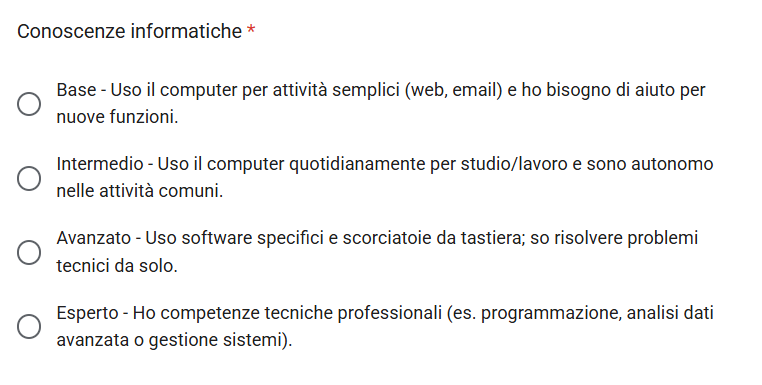
\includegraphics[width=0.8\textwidth]{./figures/05-esperimento-utenti/modulo-anagrafica/Conoscenze informatiche.png}
    \caption{Conoscenze informatiche}
    \label{fig:conoscenze-informatiche}
\end{figure}

\begin{figure}[H]
    \centering
    
\includegraphics[width=0.8\textwidth]{./figures/05-esperimento-utenti/modulo-anagrafica/uso-web.png}
    \caption{Principale uso del web}
    \label{fig:uso-web}
\end{figure}

\begin{figure}[H]
    \centering
    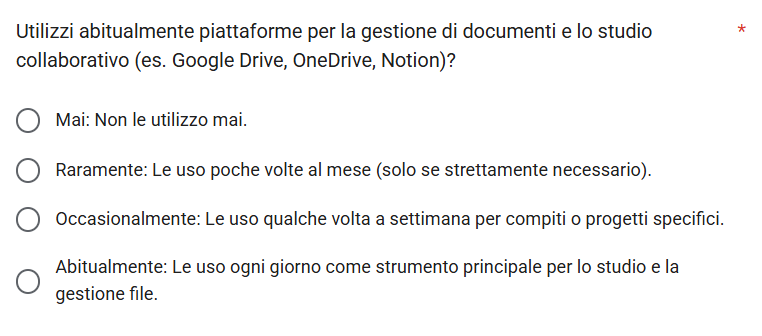
\includegraphics[width=0.8\textwidth]{./figures/05-esperimento-utenti/modulo-anagrafica/uso-ambiente-studio.png}
    \caption{Utilizzo abituale delle piattaforme di studio}
    \label{fig:utilizzo-piattaforme}
\end{figure}

\begin{figure}[H]
    \centering
    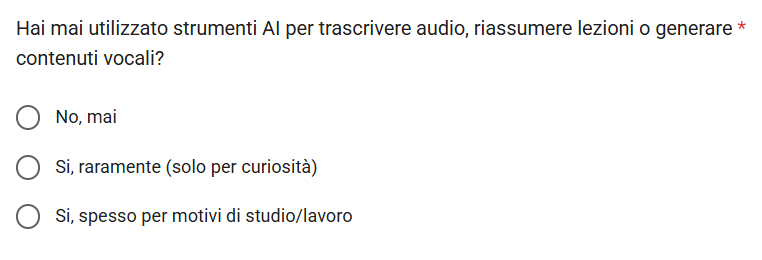
\includegraphics[width=0.8\textwidth]{./figures/05-esperimento-utenti/modulo-anagrafica/strumentiAI.png}
    \caption{Utilizzo di strumenti AI}
    \label{fig:strumentiAI}
\end{figure}

\subsubsection{Questionario di valutazione}
Terminata questa fase preliminare, l'esecuzione pratica del test è stata supportata dall'utilizzo parallelo di due ulteriori moduli, strutturati per affiancare sia il tester che l'osservatore per l'intera durata dell'esperimento. Il primo di questi è il questionario di valutazione, mantenuto aperto dall'utente durante la sessione, permetteva di leggere la descrizione dei singoli compiti (o scenari) da svolgere e di esprimere, immediatamente dopo ciascuna esecuzione, un giudizio sulla difficoltà percepita. Al termine di tutti i task, il medesimo modulo presentava il questionario SUS \textit{(System Usability Scale)} per raccogliere la valutazione complessiva dell'interfaccia (Sezione \ref{subsubsec:questionario_post_esperimento}).

\begin{figure}[H]
    \centering
    
\includegraphics[width=0.8\textwidth]{./figures/05-esperimento-utenti/questionario-valutazione/benvenuto.png}
    \caption{Nota informativa}
    \label{fig:nota-informativa}
\end{figure}

Per garantire il corretto allineamento dei dati raccolti, a ogni partecipante veniva assegnato preventivamente un codice identificativo univoco da parte dello sperimentatore. L'utente doveva inserire tale codice come prima operazione all'interno del proprio modulo (come mostrato in Figura \ref{fig:id}), permettendo così di incrociare in fase di analisi le sue valutazioni soggettive con le metriche oggettive registrate dall'osservatore.

\begin{figure}[H]
    \centering
    
\includegraphics[width=0.8\textwidth]{./figures/05-esperimento-utenti/questionario-valutazione/identificativo.png}
    \caption{Inserimento ID utente}
    \label{fig:identificativo}
\end{figure}

Per selezionare la versione del sistema da testare (A o B), era lo sperimentatore a indicare all'utente quale opzione spuntare nel modulo. Questa scelta dipendeva dal gruppo a cui era stato assegnato il tester, in modo da alternare l'ordine di esecuzione (A-B oppure B-A) e limitare l'effetto apprendimento.

Proprio come per l'identificativo, indicare la versione corretta era fondamentale per allineare il questionario dell'utente con il modulo usato dallo sperimentatore (vedi Figura \ref{fig:vers} nella sezione relativa al modulo dello sperimentatore). Grazie a questa impostazione, è stato possibile riutilizzare gli stessi moduli per testare entrambe le versioni con ciascun partecipante: dal momento che i compiti e gli scenari erano identici per entrambe le varianti del sistema, l'utente e l'osservatore compilavano semplicemente lo stesso form prima per una versione e poi per l'altra. Questo ci ha permesso di raccogliere i dati in modo coerente e di poterli confrontare facilmente.

\begin{figure}[H]
    \centering
    
\includegraphics[width=0.8\textwidth]{./figures/05-esperimento-utenti/questionario-valutazione/versione.png}
    \caption{Selezione della versione da testare}
    \label{fig:versione}
\end{figure}

Nelle figure seguenti sono riportate le schermate del modulo relative ai sei compiti e ai due scenari proposti agli utenti. Come si può notare, al termine della descrizione di ogni task è presente una specifica domanda ("Come giudichi questo compito?" oppure "Come giudichi questo scenario?"). Per esprimere la propria valutazione, il tester ha utilizzato una \textit{scala Likert a 5 punti}, dove 1 corrispondeva a \textit{Molto facile} e 5 a \textit{Molto difficile} (passando per i valori intermedi di \textit{facile}, \textit{né facile né difficile} e \textit{difficile}). È importante precisare un dettaglio fondamentale: ai tester è stato spiegato chiaramente che il giudizio richiesto non doveva riguardare la complessità intrinseca del compito o dello scenario in sé, ma doveva misurare esclusivamente quanto l'interfaccia e il sistema ne rendessero semplice o complicata l'esecuzione.

\begin{figure}[H]
    \centering
    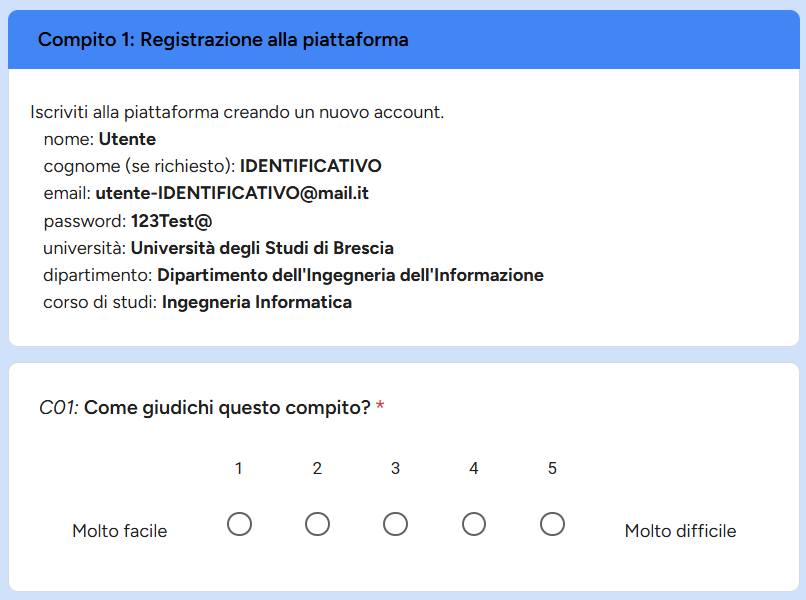
\includegraphics[width=0.8\textwidth]{./figures/05-esperimento-utenti/questionario-valutazione/compito1.png}
    \caption{Compito 1}
    \label{fig:compito1}
\end{figure}

\begin{figure}[H]
    \centering
    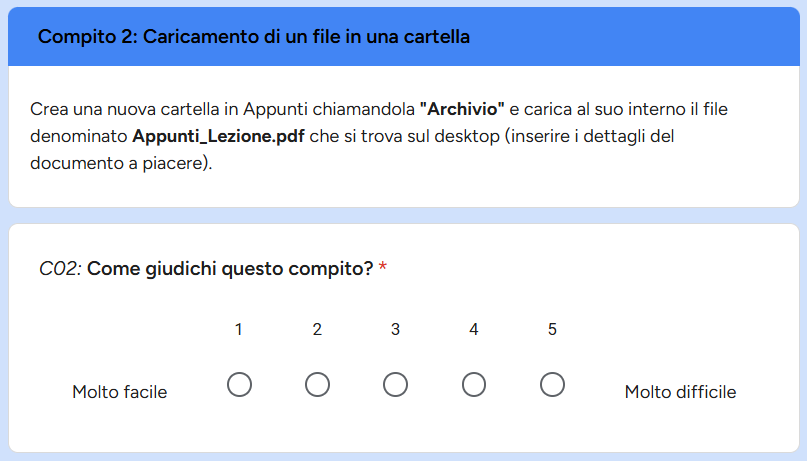
\includegraphics[width=0.8\textwidth]{./figures/05-esperimento-utenti/questionario-valutazione/compito2.png}
    \caption{Compito 2}
    \label{fig:compito2}
\end{figure}

\begin{figure}[H]
    \centering
    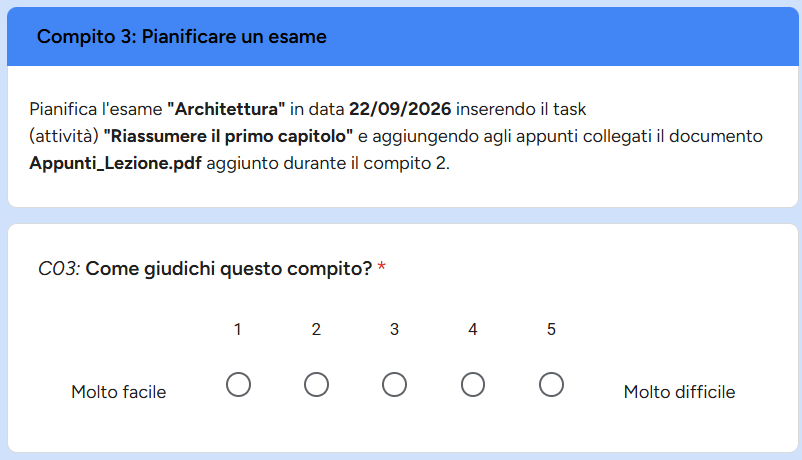
\includegraphics[width=0.8\textwidth]{./figures/05-esperimento-utenti/questionario-valutazione/compito3.png}
    \caption{Compito 3}
    \label{fig:compito3}
\end{figure}

\begin{figure}[H]
    \centering
    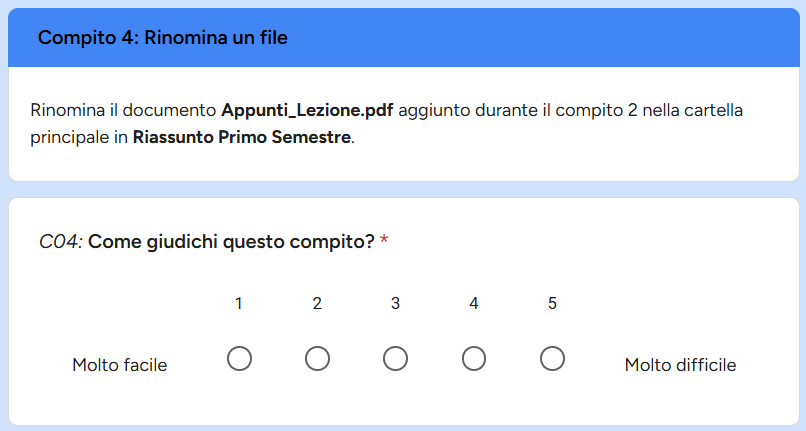
\includegraphics[width=0.8\textwidth]{./figures/05-esperimento-utenti/questionario-valutazione/compito4.png}
    \caption{Compito 4}
    \label{fig:compito4}
\end{figure}

\begin{figure}[H]
    \centering
    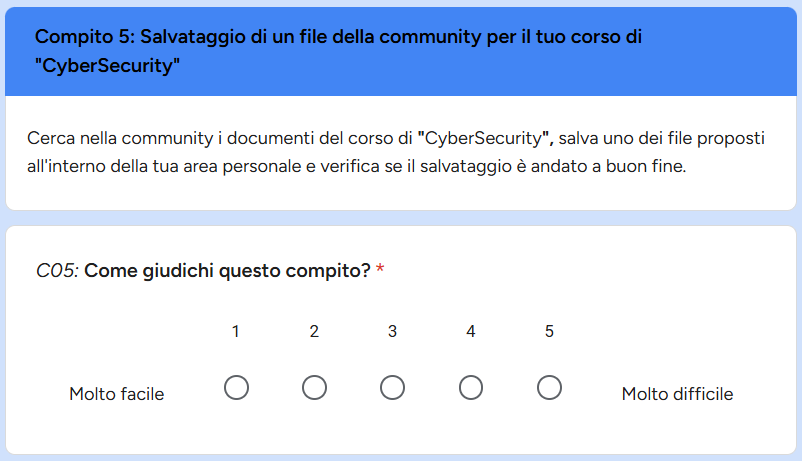
\includegraphics[width=0.8\textwidth]{./figures/05-esperimento-utenti/questionario-valutazione/compito5.png}
    \caption{Compito 5}
    \label{fig:compito5}
\end{figure}

\begin{figure}[H]
    \centering
    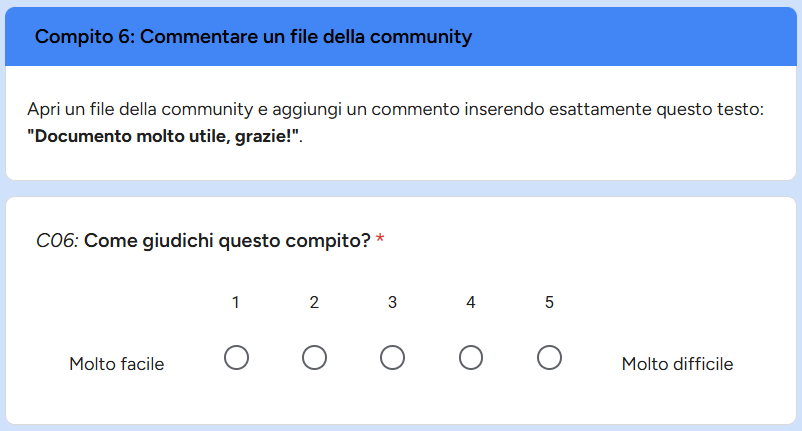
\includegraphics[width=0.8\textwidth]{./figures/05-esperimento-utenti/questionario-valutazione/compito6.png}
    \caption{Compito 6}
    \label{fig:compito6}
\end{figure}

\begin{figure}[H]
    \centering
    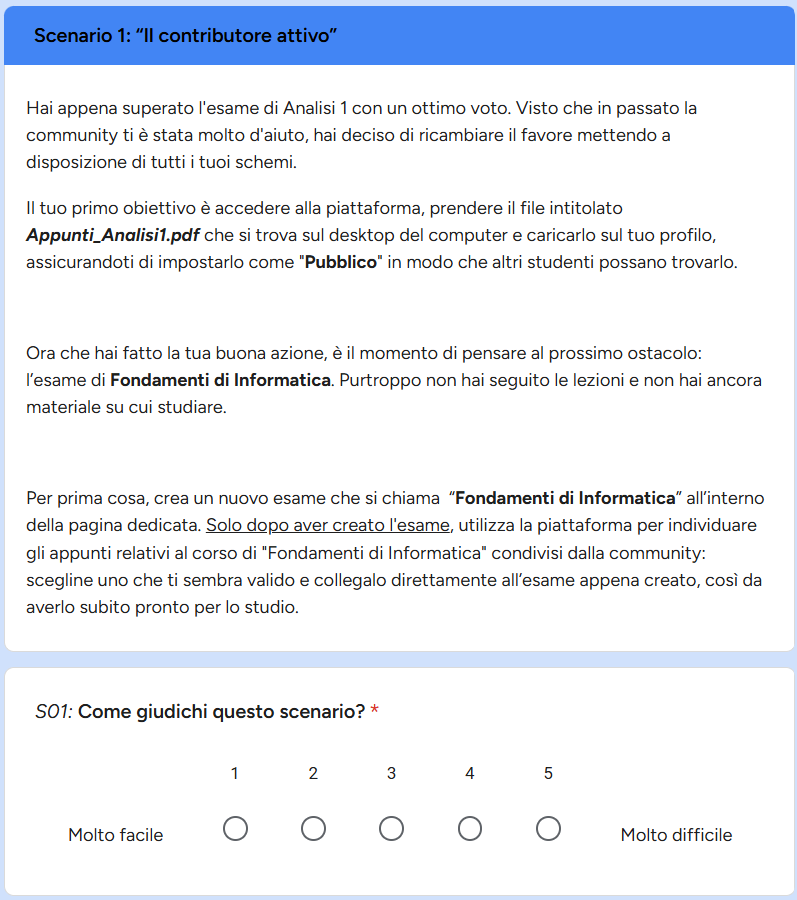
\includegraphics[width=0.8\textwidth]{./figures/05-esperimento-utenti/questionario-valutazione/scenario1.png}
    \caption{Scenario 1}
    \label{fig:scenario1}
\end{figure}

\begin{figure}[H]
    \centering
    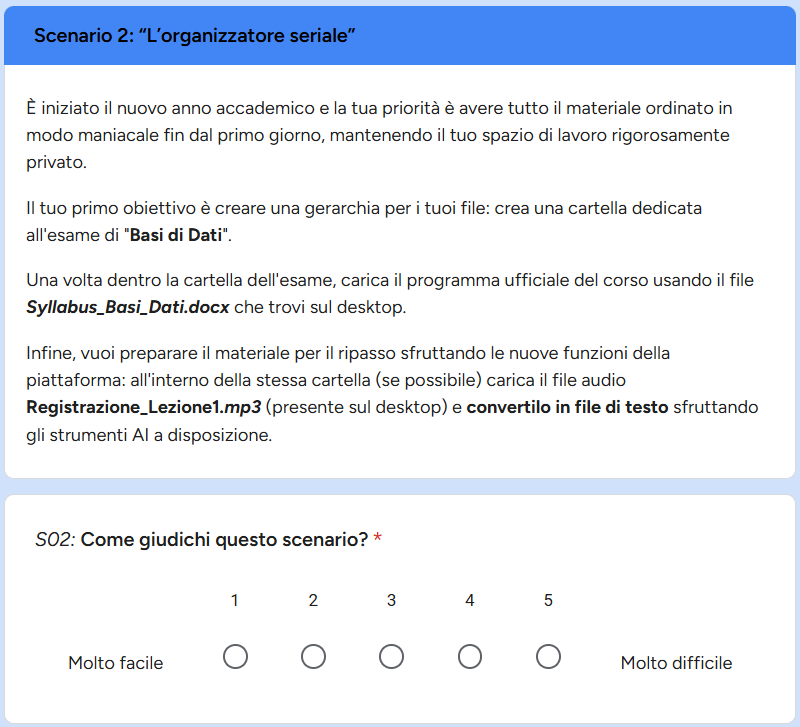
\includegraphics[width=0.8\textwidth]{./figures/05-esperimento-utenti/questionario-valutazione/scenario2.png}
    \caption{Scenario 2}
    \label{fig:scenario2}
\end{figure}

\subsubsection{Modulo per lo sperimentatore}
Come descritto in precedenza, le prime due sezioni di questo modulo (Figura \ref{fig:id} e Figura \ref{fig:vers}) riprendono esattamente l'inserimento dell'identificativo utente (Figura \ref{fig:identificativo}) e la selezione della versione (Figura \ref{fig:versione}), garantendo così il perfetto allineamento con il questionario compilato dal tester.

\begin{figure}[H]
    \centering
    
\includegraphics[width=0.8\textwidth]{./figures/05-esperimento-utenti/modulo-sperimentatore/identificativo}
    \caption{Inserimento ID utente}
    \label{fig:id}
\end{figure}

\begin{figure}[H]
    \centering
    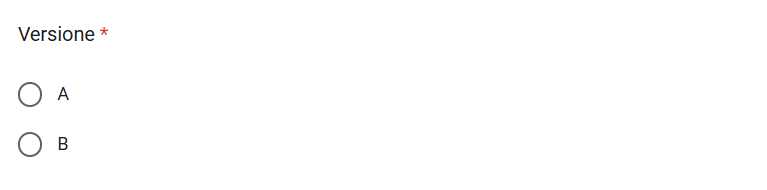
\includegraphics[width=0.8\textwidth]{./figures/05-esperimento-utenti/modulo-sperimentatore/versione}
    \caption{Selezione della versione da testare}
    \label{fig:vers}
\end{figure}

Successivamente, il modulo si struttura per singoli compiti e scenari ed è stato impiegato dall'osservatore per registrare i dati dell'esperimento. Nello specifico, la durata di esecuzione e il numero di click effettuati sono stati misurati tramite appositi tool del browser, avviati all'inizio di ogni task e azzerati prima di intraprendere quello successivo. Al termine di ciascun compito, e prima di procedere con il seguente, lo sperimentatore provvedeva ad annotare tali metriche sul modulo, integrandole con il numero di errori commessi, l'esito dell'azione, le proprie osservazioni e gli eventuali commenti espressi dall'utente.

\begin{figure}[H]
    \centering
    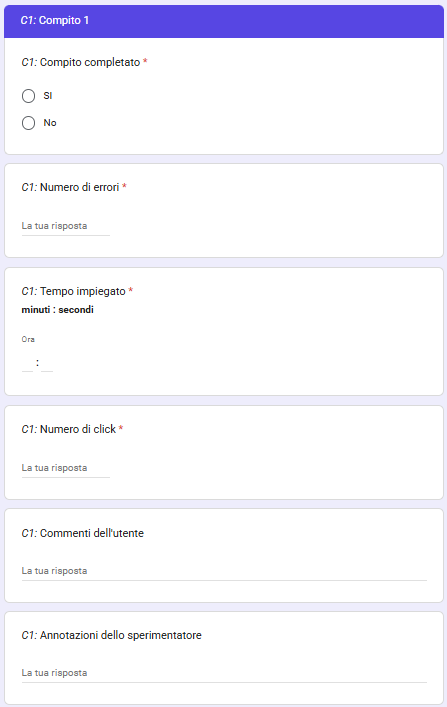
\includegraphics[width=0.7\textwidth]{./figures/05-esperimento-utenti/modulo-sperimentatore/compito1}
    \caption{Compito 1}
    \label{fig:c1}
\end{figure}

\begin{figure}[H]
    \centering
    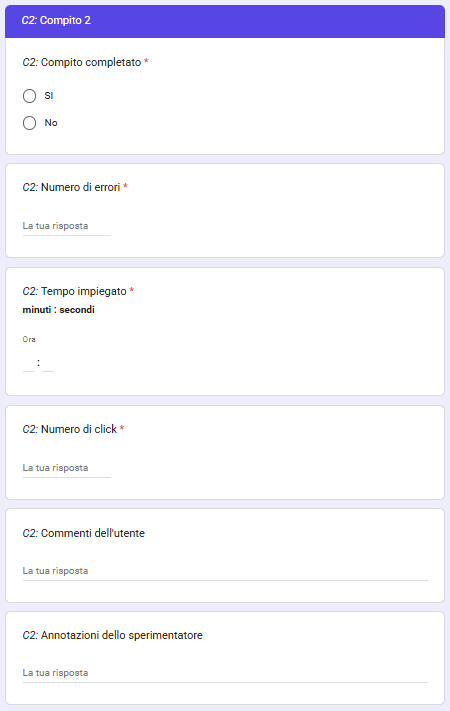
\includegraphics[width=0.7\textwidth]{./figures/05-esperimento-utenti/modulo-sperimentatore/compito2}
    \caption{Compito 2}
    \label{fig:c2}
\end{figure}

\begin{figure}[H]
    \centering
    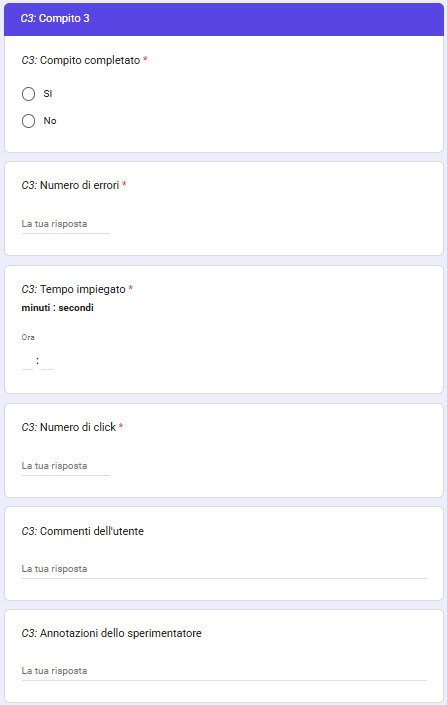
\includegraphics[width=0.7\textwidth]{./figures/05-esperimento-utenti/modulo-sperimentatore/compito3}
    \caption{Compito 3}
    \label{fig:c3}
\end{figure}

\begin{figure}[H]
    \centering
    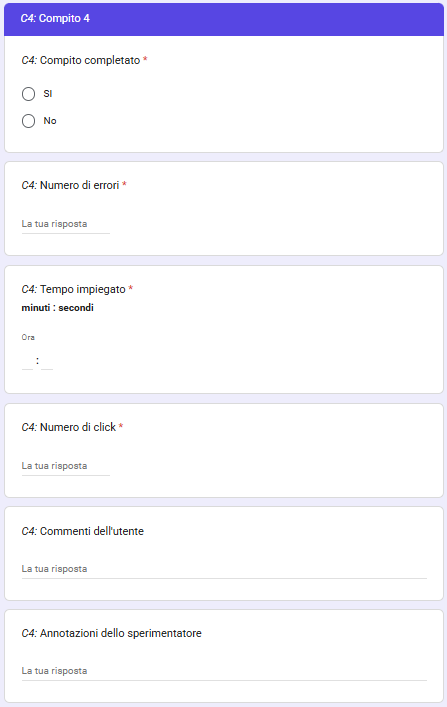
\includegraphics[width=0.7\textwidth]{./figures/05-esperimento-utenti/modulo-sperimentatore/compito4}
    \caption{Compito 4}
    \label{fig:c4}
\end{figure}

\begin{figure}[H]
    \centering
    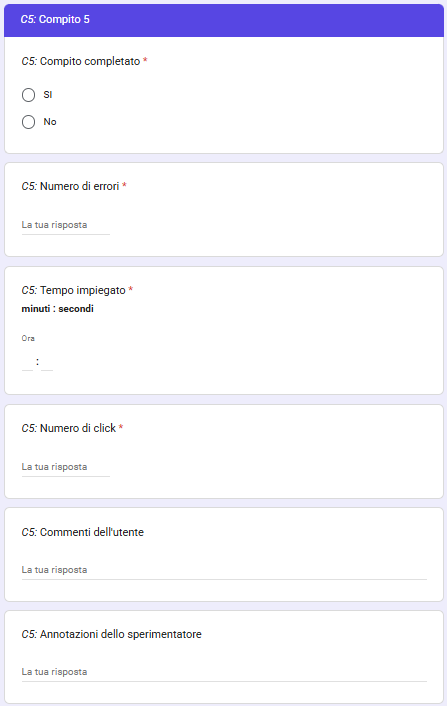
\includegraphics[width=0.7\textwidth]{./figures/05-esperimento-utenti/modulo-sperimentatore/compito5}
    \caption{Compito 5}
    \label{fig:c5}
\end{figure}

\begin{figure}[H]
    \centering
    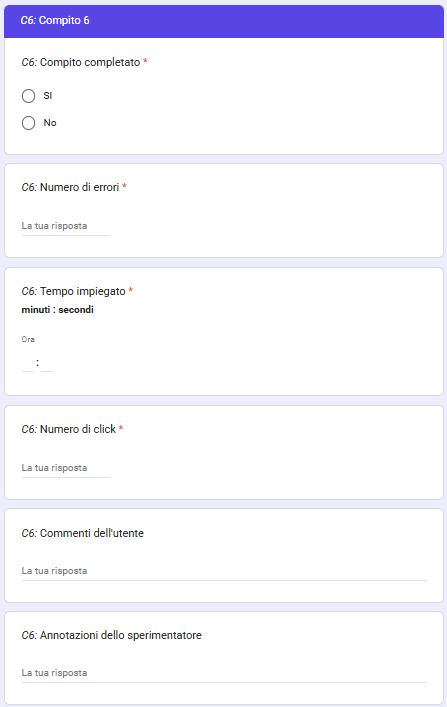
\includegraphics[width=0.7\textwidth]{./figures/05-esperimento-utenti/modulo-sperimentatore/compito6}
    \caption{Compito 6}
    \label{fig:c6}
\end{figure}

\begin{figure}[H]
    \centering
    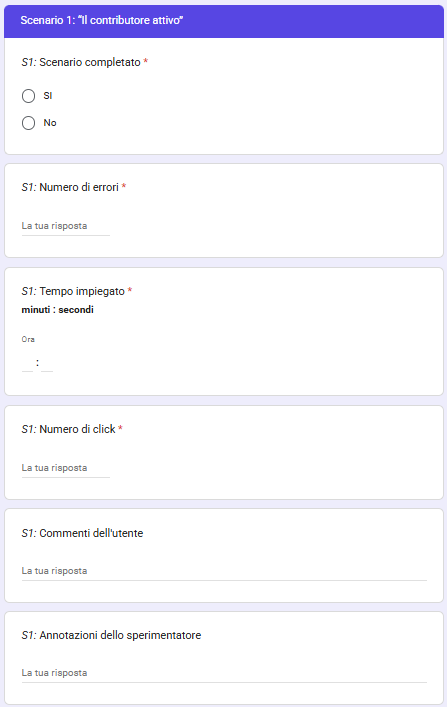
\includegraphics[width=0.7\textwidth]{./figures/05-esperimento-utenti/modulo-sperimentatore/scenario1}
    \caption{Scenario 1}
    \label{fig:s1}
\end{figure}

\begin{figure}[H]
    \centering
    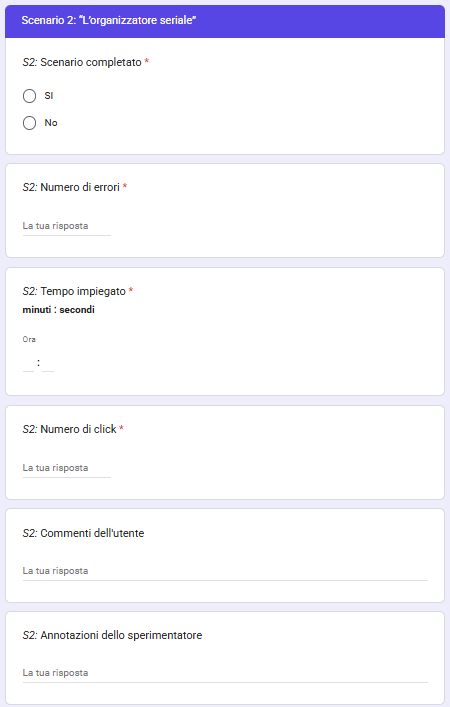
\includegraphics[width=0.7\textwidth]{./figures/05-esperimento-utenti/modulo-sperimentatore/scenario2}
    \caption{Scenario 2}
    \label{fig:s2}
\end{figure}

\subsubsection{Questionario post-esperimento}
\label{subsubsec:questionario_post_esperimento}

Al termine della sessione di test di ciascuna versione, è stato sottoposto all'utente un questionario post-esperimento per raccogliere un giudizio complessivo sull'interazione appena conclusa. Per questa fase di valutazione si è scelto di adottare il questionario SUS (\textit{System Usability Scale}), essendo uno standard ampiamente consolidato nel settore. Questo strumento propone un set di dieci affermazioni generiche e indipendenti dal dominio, rivelandosi quindi adatto a valutare qualsiasi tipologia di sistema o interfaccia. Una caratteristica peculiare del SUS è la sua struttura: per mantenere alta l'attenzione del tester ed evitare risposte meccaniche, il questionario alterna cinque affermazioni formulate in positivo a cinque formulate in negativo. Per ciascuna voce, il partecipante è chiamato a esprimere il proprio grado di accordo o disaccordo avvalendosi di una \textit{scala Likert a 5 punti} (da "Fortemente in disaccordo" a "Fortemente in accordo"). Il principale vantaggio di questo questionario risiede nella sua capacità di sintetizzare le risposte in un unico punteggio numerico: tale valore costituisce un indicatore globale dell'usabilità percepita, rendendo possibile un confronto oggettivo sia tra le due versioni testate, sia rispetto a un valore di riferimento. Per i dettagli sul metodo di calcolo effettivo del punteggio e per la relativa valutazione, si rimanda alla Sezione \ref{sec:tua_sezione_analisi}.

\begin{figure}[H]
    \centering
    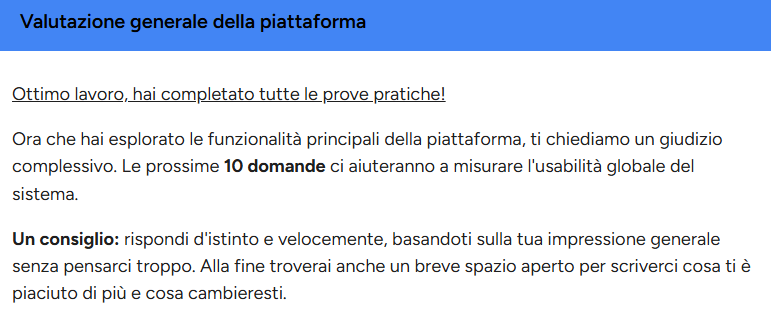
\includegraphics[width=0.8\textwidth]{./figures/05-esperimento-utenti/questionario-SUS/info-SUS.png}
    \caption{Nota informativa}
    \label{fig:info-SUS}
\end{figure}

\begin{figure}[H]
    \centering
    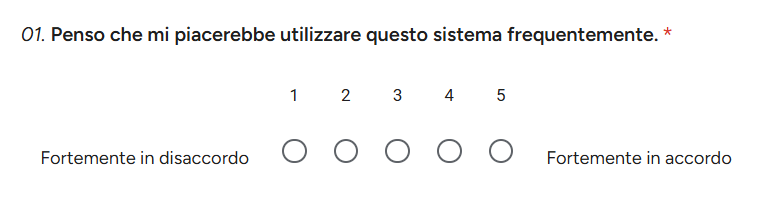
\includegraphics[width=0.8\textwidth]{./figures/05-esperimento-utenti/questionario-SUS/dom1.png}
    \caption{Affermazione 1}
    \label{fig:dom1}
\end{figure}

\begin{figure}[H]
    \centering
    
\includegraphics[width=0.8\textwidth]{./figures/05-esperimento-utenti/questionario-SUS/dom2.png}
    \caption{Affermazione 2}
    \label{fig:dom2}
\end{figure}

\begin{figure}[H]
    \centering
    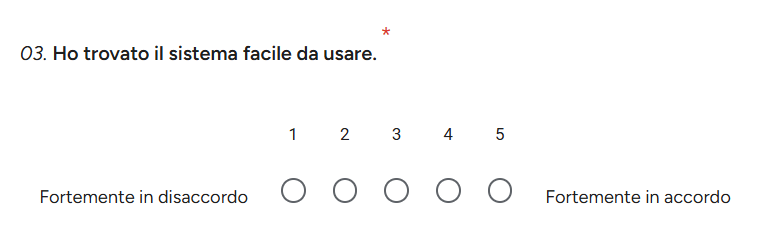
\includegraphics[width=0.8\textwidth]{./figures/05-esperimento-utenti/questionario-SUS/dom3.png}
    \caption{Affermazione 3}
    \label{fig:dom3}
\end{figure}

\begin{figure}[H]
    \centering
    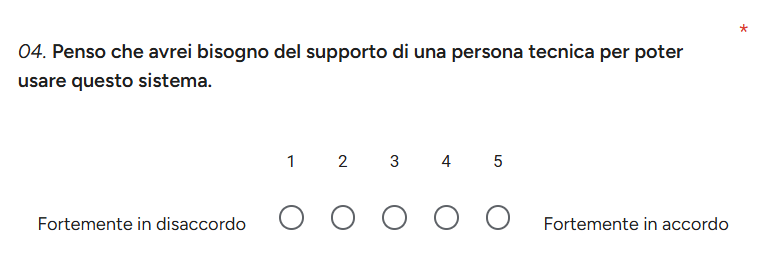
\includegraphics[width=0.8\textwidth]{./figures/05-esperimento-utenti/questionario-SUS/dom4.png}
    \caption{Affermazione 4}
    \label{fig:dom4}
\end{figure}

\begin{figure}[H]
    \centering
    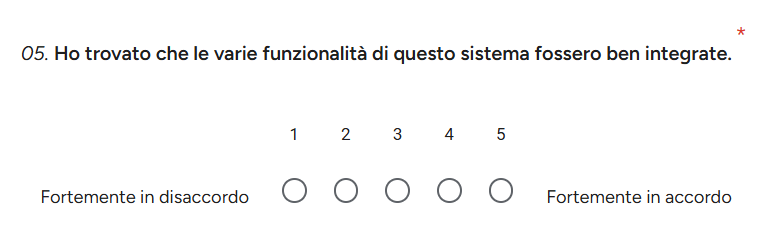
\includegraphics[width=0.8\textwidth]{./figures/05-esperimento-utenti/questionario-SUS/dom5.png}
    \caption{Affermazione 5}
    \label{fig:dom5}
\end{figure}

\begin{figure}[H]
    \centering
    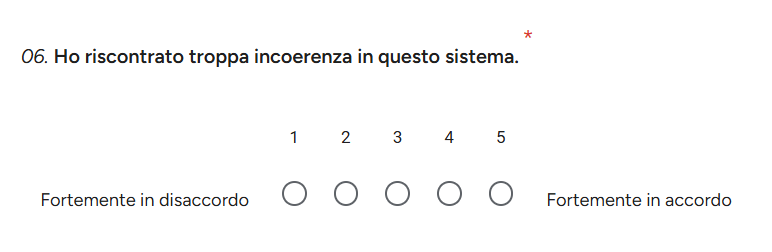
\includegraphics[width=0.8\textwidth]{./figures/05-esperimento-utenti/questionario-SUS/dom6.png}
    \caption{Affermazione 6}
    \label{fig:dom6}
\end{figure}

\begin{figure}[H]
    \centering
    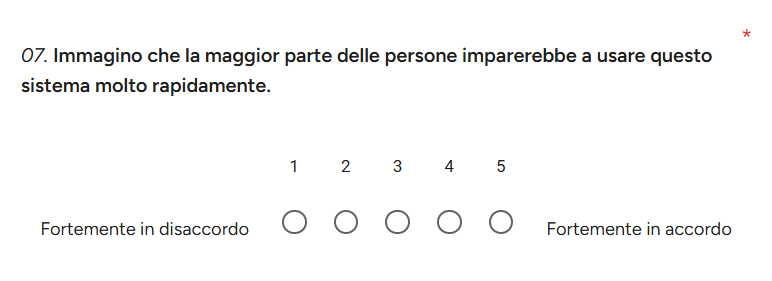
\includegraphics[width=0.8\textwidth]{./figures/05-esperimento-utenti/questionario-SUS/dom7.png}
    \caption{Affermazione 7}
    \label{fig:dom7}
\end{figure}

\begin{figure}[H]
    \centering
    
\includegraphics[width=0.8\textwidth]{./figures/05-esperimento-utenti/questionario-SUS/dom8.png}
    \caption{Affermazione 8}
    \label{fig:dom8}
\end{figure}

\begin{figure}[H]
    \centering
    
\includegraphics[width=0.8\textwidth]{./figures/05-esperimento-utenti/questionario-SUS/dom9.png}
    \caption{Affermazione 9}
    \label{fig:dom9}
\end{figure}

\begin{figure}[H]
    \centering
    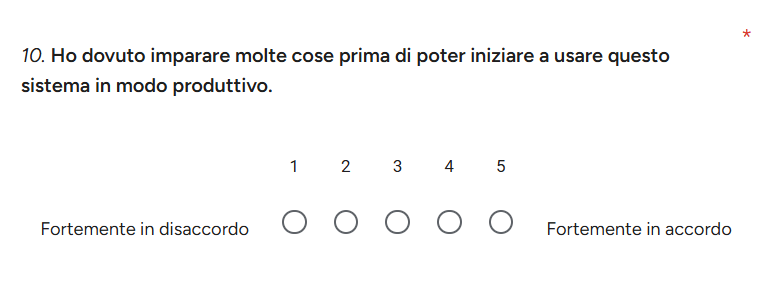
\includegraphics[width=0.8\textwidth]{./figures/05-esperimento-utenti/questionario-SUS/dom10.png}
    \caption{Affermazione 10}
    \label{fig:dom10}
\end{figure}

Infine, a chiusura del modulo, è stata predisposta un'ulteriore sezione a compilazione facoltativa (come visibile in Figura \ref{fig:impressioni}), dedicata alla raccolta di eventuali commenti, impressioni generali o suggerimenti spontanei dell'utente in merito all'intero sistema.

\begin{figure}[H]
    \centering
    
\includegraphics[width=0.8\textwidth]{./figures/05-esperimento-utenti/questionario-SUS/impressioni-generali.png}
    \caption{Inserimento impressioni generali dell'utente}
    \label{fig:impressioni}
\end{figure}

\subsubsection{Links ai moduli}
Per completezza, si riportano i collegamenti ai moduli utilizzati:
\begin{itemize}
    \item \textbf{Modulo Anagrafica:} \url{https://forms.gle/W9ce9BewdVnGAwJG8}
    \item \textbf{Questionario di valutazione:} \url{https://forms.gle/owEJTn2Dgkx1qrcp6}
    \item \textbf{Modulo per lo sperimentatore:} \url{https://forms.gle/uS6dAbXeJvTRN45d9}
\end{itemize}